%% This document gives an example on how to use the ntnumasterthesis
%% LaTeX document class.

%% Use short name MACS, MIS, CIMET, MTDMT, MIXD or MIS  
%% Language english or norsk
%% b5paper with oneside or twoside, you can set A4 if you want but you submit in b5

%% If you want print with the heading material on a4 paper you can use this format
%% \documentclass[MACS,english,a4paper,oneside,12pt]{ntnuthesis/ntnuthesis}

%% with the change to using DAIM we have a new option. include DAIM after english below removes the front page material so that you can then submit in the DAIM system. If you are wanting the front material remove DAIM and make sure you fill in the DaimData.tex file.
\documentclass[MIS,english]{ntnuthesis/ntnuthesis}

\usepackage[T1]{fontenc}
\usepackage[utf8]{inputenc}     % For utf8 encoded .tex files allows norwegian characters in the files. This can be dangerous if you change to a differnt editor.
%\usepackage[pdftex]{graphicx, hyperref}   % For cross references in pdf
\usepackage{graphicx}
\usepackage{hyperref}   % For cross references in pdf

% For smart references 
%    use \cref{label} and Caption and Number will be added automatically
\usepackage[capitalise,noabbrev]{cleveref} 

\usepackage{color}              % For colouring text 
\hypersetup{colorlinks=true,     
		linkcolor=blue,          % color of internal links (change box color with linkbordercolor)
    citecolor=blue,        % color of links to bibliography
    filecolor=blue,      % color of file links
    urlcolor=blue           % color of external links
		}
\usepackage{csvsimple}  % for simple table reading and display
\usepackage{url}
\usepackage{booktabs}
\usepackage{gnuplottex} %miktex option if using miktex on windows
\usepackage{rotating}


\definecolor{darkgreen}{rgb}{0,0.5,0}
\definecolor{darkred}{rgb}{0.5,0.0,0}

\lstset{        basicstyle=\ttfamily,
                keywordstyle=\color{blue}\ttfamily,
                stringstyle=\color{darkred}\ttfamily,
                commentstyle=\color{darkgreen}\ttfamily,
}


%Typesetting of C++ but not always stable in titles etc...
\newcommand{\CPP}[0]{{C\nolinebreak[4]\hspace{-.1em}\raisebox{.1ex}{\small\bf +\hspace{-.1em}+\ }}}

%\usepackage[table]{xcolor}% http://ctan.org/pkg/xcolor
%\usepackage[nomessages]{fp}
%\newlength{\maxbarlen}


\newcommand\databar[3][gray!20]{%
  \FPeval\result{round(#3/#2:4)}%
  \rlap{\textcolor{#1}{\hspace*{\dimexpr-\tabcolsep+.5\arrayrulewidth}%
        \rule[-.05\ht\strutbox]{\result\maxbarlen}{.95\ht\strutbox}}}%
  \makebox[\dimexpr\maxbarlen-2\tabcolsep+\arrayrulewidth][r]{#3}}



\newcommand{\com}[1]{{\color{red}#1}} % supervisor comment
%\renewcommand{\com}[1]{} %remove starting % to remove supervisor comments
% This will appear in text \com{Lecuters comment} and be visible unless you uncomment
% the renewcommand line.

\newcommand{\todo}[1]{{\color{green}#1}} % items to do
%\renewcommand{\todo}[1]{} %remove starting % to remove items to do

\newcommand{\n}[1]{{\color{blue}#1}} % other comment
%\renewcommand{\n}[1]{} %remove starting % to remove notes

\newcommand{\dn}[1]{} % add the d to a note to say that you have finished with it.





% Set to true ONLY if using Harvard citation style
\newboolean{HarvardCitations}
\setboolean{HarvardCitations}{false} % false for computer science, true for interaction design and harvard style


\ifthenelse{\boolean{HarvardCitations}}{%
	\usepackage{natbib} % for Harvard names as citations.
}{%
	\usepackage[numbers]{natbib} % for Vancover numbers in bibliography
}

\newcommand{\q}[1]{\leavevmode\marginpar{\small\em #1}}
\renewcommand{\q}[1]{}


\begin{document}

% for students submitting in the DAIM system this information will not be used.
% their is an option for DAIM submission which removes this information and checks it is B5.
% Removing the DAIM option on the document type will use this material.

\setthesistitle{Real Time Windows Event Log Analysis}
\setthesisshorttitle{Real Time Windows Event Log Analysis} % a short version for the page headers if your normal title is too long to fit
\setthesisauthor{Martin Ingesen}
\setthesissupervisor{Prof. ?}
\setthesissupervisorA{Prof. ?}  % if you have a second supervisor add it like this
%\setthesissupervisorB{Prof. Smart Guy}  % if you have a second supervisor add it like this


\nmtkeywords{Thesis, Latex, Template, IMT}
%\nmtdesc{This is the short description of a masters thesis}


\setthesisdate{12-12-2019}
\setthesisyear{2019}



%for CIMET theses you need to see all of these as well

%\setthesiscampus{Gj\o{}vik}
%\setthesisHostInstitution{\NTNU}
%\setthesisHostInstitution{University of Eastern Finland}
%\setthesisHostInstitution{Universit\'e Jean Monnet Saint-Etienne}

%\setthesisjuryA{} %jury names
%\setthesisjuryB{} %jury names
%\setthesisjuryC{} %jury names
%\setthesisjuryD{} %jury names


 % this is the file which contains all the details about your thesis
\makefrontpages % make the frontpages
%this is the intro to the thesis
\include{inc/preface}

\include{inc/acknowledgments}

\include{inc/abstract}


\tableofcontents

\hypersetup{pageanchor=true}

% Comment with a percent to remove figures or tables:
\listoffigures
\listoftables
\lstlistoflistings


\chapter{Introduction}
\label{chap:introduction}

\iffalse
Scrutiny of the introduction - http://sepwww.stanford.edu/sep/prof/Intro.html
\fi

\iffalse
The review

Pick out about 3-10 papers providing a background to your research and say something about each of them. You could paraphrase a sentence or two from each abstract. The review is not intended to be a historical review going back to Newton or Descartes. Try to find a few papers by your office mates, your advisor, your predecessors, or other associates. That way you might find somebody to give you helpful criticism!

Anyone can follow these instructions and write a review that looks presentable. Where intelligence and skill are required is in organizing the review so that it leads up to something, namely, to your claim.
\fi

\iffalse
The claim

The most important part of the introduction is buried in the middle. It is the claim. The claim is where you claim your work is a worthwhile extension of the review you just wrote. If someone says your writing is "unmotivated," they are not insulting your humanity; it just means they can't find your claim.

In your claim you should use the personal pronoun "I" (or "we" if you aren't the sole author). The word "I" tells people where common knowledge runs out and your ideas begin. If you are writing a doctoral dissertation or an article for a refereed journal, then you should be making a new contribution to existing knowledge. Your paper is not acceptable without an identifiable claim.
\fi

\iffalse
I believe that by using a more modern pipeline, programming language and ruleset for event correlation, we can improve not just the correlation throughput (events per second), but also make it simpler for security analysts to create, edit and manage correlation rules.
\fi

\iffalse
The agenda

An agenda is found at the end of many introductions. It summarizes what you will show the reader as your paper progresses. Your agenda will be dull if it is merely a recital of the topics you will cover. Your agenda should tell how your paper works to fulfill your claim. In this way your agenda should clarify your claim.

The agenda is not as important as the review and the claim. Keep it short.

Occasionally you will be fortunate enough to be writing about something in which some of your conclusions can be made in simple statements. If so, state them early, right after your agenda. You aren't trying to write a mystery! Many more people will begin reading your paper than will finish reading it. Motivate them to finish! Unfortunately, many technical papers do not lend themselves to early conclusions.
\fi
\iffalse
In this thesis, I will first give some background into the field of correlating event technologies, and give an overview of the state-of-the-art. Then I will explain the methods I have used to measure and analyze our results. After this, I will go into detail on our results, before we then discuss and analyse our results. Finally, I will conclude with some further work to be done.


\makebox[\linewidth]{\rule{\paperwidth}{0.4pt}}
\fi

This field is maturing, as focus has shifted from network monitoring and detection, to a more endpoint-centric approach....

\section{Problem description}
\label{sec:problemdescription}

We are seeing a movement away from network-based monitoring and detection. There are several reasons for this.

\begin{itemize}
    \item Increased usage of encrypted communications, as encryption has become standard and more popular than ever before. The continued introduction of other privacy-enhancing technologies like DNS-over-TLS/DNS-over-HTTPS will continue to hinder network-based monitoring and detection from being effective.
    \item Endpoints are no longer static inside a business network. Employees bring the computers with them outside of the office. Sometimes connected to their business' network via a Virtual Private Network (VPN), sometimes not.
    \item Network-based detection only give you a glimpse at what happens on the wire. There is not visibility into what is happening on the individual endpoints connected to the network.
\end{itemize}
The trend seems to be moving more towards host-based monitoring and detection instead. Traditionally, this has been frowned upon, as CPU-intensive agents would have to be installed on the endpoints. But now we are seeing higher performing agents, as well endpoints with more performant hardware. There are several advantages to moving to endpoint monitoring and detection.

\begin{itemize}
    \item Host-based detection and response makes it easier to detect anomalies and badness using either 3rd party software, or built-in capabilities of the OS.
    \item We are not bound to a particular network for protection, so we are still covered monitoring and detection-wise when on the move.
    \item There is a constant development to allow further insight into what is happening on the endpoint by the OS-vendors.
\end{itemize}

Current detection analysis is based on aggregating log files into a centralized system known as a System Information and Event Management (SIEM) system. Traditionally in a SIEM, logs are analyzed after-the-fact. This has several drawbacks:

\begin{itemize}
    \item Security monitoring is reactive.
    \item Requires actively hunting for bad events.
\end{itemize}

Another huge problem with pure SIEM-based logging, as companies are collecting more and more logs, actively hunting for badness in those logs are becoming harder and more complex. I single log item from a single source is not enough to properly analyze what has happened in a system. Only by cross-correlating several log lines and log sources are we able fully understand the situation at hand.

An example of this might be that we have a log item X. This means Y and is not a indication of badness in and of itself.
But if we also see log item Y right before log item X, that could be a indication of attack-pattern X. Which is a known Indicator of Compromise.



\iffalse
FROM http://folk.uio.no/josang/papers/MJ2018-ICCSP.pdf
Current threat detection analysis approaches include aggregation of log files in a centralized system known as security information and event management (SIEM) which performs inspections
and flags anomalies. A SIEM system collects logs by deploying
multiple collection agents to gather security-related events from
end-user devices, servers, intrusion detection systems (IDS), intrusion prevention systems (IPS) and firewalls, network devices such as
routers and DNS servers and more. In particular, one resource that
has received considerable attention for endpoint visibility has been
Sysmon; a Windows system service and device driver that monitors
and logs system activity of Windows workstations. Approaches for
threat detection using Sysmon have been proposed mainly focusing
on search engines (NoSQL database systems) or graph databases.
\fi

\section{Justification, motivation and benefits}
\label{sec:justificationmotivationandbenefits}
...
There are several benefits of this approach. We are using more modern, industry-standard technology which improves scalability, availability and performance.

\section{Research questions}
\label{sec:researchquestions}

\begin{itemize}
\item How can we improve event correlation/the SEC algorithm...? Hvordan kan vi forbedre event log analyse?
Implementerer en mer effektiv versjon.
    \item How can we make event log analysis and correlation faster using a compiled programming language (Go) rather than a dynamic, interpreted language like Perl.
    \item How can we make event log correlation simpler for the analyst by utilizing a common alert format for writing and sharing rules, instead of the heavily regular expression-based apporach of SEC?
    \item How can we further improve the distributed nature of log ingestion and processing by using queuing technologies and a shared in-memory cache for context-information between the event analyzers.
    \item Does correlating events reduce the number of false positives, and therefore avoid "alert fatigue"?
\end{itemize}

\section{Planned contributions}
\label{sec:plannedcontributions}

This thesis will:

\begin{itemize}
    \item Implement and detail a system for correlating Windows Event Logs in near real time. Using Go.
    \item Analyze benefits and drawbacks of using our system versus other tools.
    \item Show how the system performs on real world data, with a focus on measures to reduce the number of false positives.
    \item Contribute rules for common attack techniques back to the community, that require correlation to avoid a high false-positive rate.
\end{itemize}


\section{Thesis Outline}
\label{sec:thesisoutline}

First, we will.... % includes latex files from the same directory
\chapter{Literature review}
\label{chap:literaturereview}

\chapter{Implementation}
\label{chap:implementation}
This has the description of how you actually went about implementing the project.  This should be focused on the interesting challenges and how those related to the project.

\todo{add more here}

\begin{figure}[h]  %t top, b bottom, p page | you can also use h to try to get the figure to appear at the current location
  \centering
  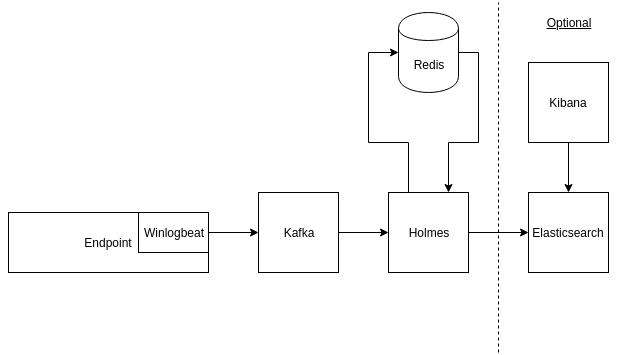
\includegraphics[width=.85\textwidth]{figures/holmes-architecture}
  \caption[An example figure.]{Minimal architecture. Every single node can be scaled both vertically and horizontally.}
  \label{fig:example}
\end{figure}
\iffalse
\include{inc/packages} % could be called Methodology or methods or any filename 
\include{inc/structure} % could be results
\chapter{Discussion}
\label{chap:discussion}

\section{Limitations of the study}
\label{sec:limitations}

\section{Future work}
\label{sec:futurework}

\todo{What could be expanded further upon in the future?}
\todo{Are there any experiments that we could have done, but didn't have the time to do? What could they tell us that we already didn't know?}
\chapter{Conclusion}
\label{chap:conclusion}
\fi
\ifthenelse{\boolean{HarvardCitations}}{%
	\bibliographystyle{agsm} % used for Harvard style references. Names - Humanities & Interaction Design
}{%
	\bibliographystyle{ntnuthesis/ntnuthesis} %used for Vancover style references. Numbers - Computer Science & Physics
}

\bibliography{MastersExample}

\appendix
\include{inc/rawdata}

\end{document}
